% Options for packages loaded elsewhere
\PassOptionsToPackage{unicode}{hyperref}
\PassOptionsToPackage{hyphens}{url}
%
\documentclass[
]{article}
\usepackage{lmodern}
\usepackage{amssymb,amsmath}
\usepackage{ifxetex,ifluatex}
\ifnum 0\ifxetex 1\fi\ifluatex 1\fi=0 % if pdftex
  \usepackage[T1]{fontenc}
  \usepackage[utf8]{inputenc}
  \usepackage{textcomp} % provide euro and other symbols
\else % if luatex or xetex
  \usepackage{unicode-math}
  \defaultfontfeatures{Scale=MatchLowercase}
  \defaultfontfeatures[\rmfamily]{Ligatures=TeX,Scale=1}
\fi
% Use upquote if available, for straight quotes in verbatim environments
\IfFileExists{upquote.sty}{\usepackage{upquote}}{}
\IfFileExists{microtype.sty}{% use microtype if available
  \usepackage[]{microtype}
  \UseMicrotypeSet[protrusion]{basicmath} % disable protrusion for tt fonts
}{}
\makeatletter
\@ifundefined{KOMAClassName}{% if non-KOMA class
  \IfFileExists{parskip.sty}{%
    \usepackage{parskip}
  }{% else
    \setlength{\parindent}{0pt}
    \setlength{\parskip}{6pt plus 2pt minus 1pt}}
}{% if KOMA class
  \KOMAoptions{parskip=half}}
\makeatother
\usepackage{xcolor}
\IfFileExists{xurl.sty}{\usepackage{xurl}}{} % add URL line breaks if available
\IfFileExists{bookmark.sty}{\usepackage{bookmark}}{\usepackage{hyperref}}
\hypersetup{
  pdftitle={1 model development},
  pdfauthor={Ing. Peter Tomko, M.A.},
  hidelinks,
  pdfcreator={LaTeX via pandoc}}
\urlstyle{same} % disable monospaced font for URLs
\usepackage[margin=1in]{geometry}
\usepackage{color}
\usepackage{fancyvrb}
\newcommand{\VerbBar}{|}
\newcommand{\VERB}{\Verb[commandchars=\\\{\}]}
\DefineVerbatimEnvironment{Highlighting}{Verbatim}{commandchars=\\\{\}}
% Add ',fontsize=\small' for more characters per line
\usepackage{framed}
\definecolor{shadecolor}{RGB}{248,248,248}
\newenvironment{Shaded}{\begin{snugshade}}{\end{snugshade}}
\newcommand{\AlertTok}[1]{\textcolor[rgb]{0.94,0.16,0.16}{#1}}
\newcommand{\AnnotationTok}[1]{\textcolor[rgb]{0.56,0.35,0.01}{\textbf{\textit{#1}}}}
\newcommand{\AttributeTok}[1]{\textcolor[rgb]{0.77,0.63,0.00}{#1}}
\newcommand{\BaseNTok}[1]{\textcolor[rgb]{0.00,0.00,0.81}{#1}}
\newcommand{\BuiltInTok}[1]{#1}
\newcommand{\CharTok}[1]{\textcolor[rgb]{0.31,0.60,0.02}{#1}}
\newcommand{\CommentTok}[1]{\textcolor[rgb]{0.56,0.35,0.01}{\textit{#1}}}
\newcommand{\CommentVarTok}[1]{\textcolor[rgb]{0.56,0.35,0.01}{\textbf{\textit{#1}}}}
\newcommand{\ConstantTok}[1]{\textcolor[rgb]{0.00,0.00,0.00}{#1}}
\newcommand{\ControlFlowTok}[1]{\textcolor[rgb]{0.13,0.29,0.53}{\textbf{#1}}}
\newcommand{\DataTypeTok}[1]{\textcolor[rgb]{0.13,0.29,0.53}{#1}}
\newcommand{\DecValTok}[1]{\textcolor[rgb]{0.00,0.00,0.81}{#1}}
\newcommand{\DocumentationTok}[1]{\textcolor[rgb]{0.56,0.35,0.01}{\textbf{\textit{#1}}}}
\newcommand{\ErrorTok}[1]{\textcolor[rgb]{0.64,0.00,0.00}{\textbf{#1}}}
\newcommand{\ExtensionTok}[1]{#1}
\newcommand{\FloatTok}[1]{\textcolor[rgb]{0.00,0.00,0.81}{#1}}
\newcommand{\FunctionTok}[1]{\textcolor[rgb]{0.00,0.00,0.00}{#1}}
\newcommand{\ImportTok}[1]{#1}
\newcommand{\InformationTok}[1]{\textcolor[rgb]{0.56,0.35,0.01}{\textbf{\textit{#1}}}}
\newcommand{\KeywordTok}[1]{\textcolor[rgb]{0.13,0.29,0.53}{\textbf{#1}}}
\newcommand{\NormalTok}[1]{#1}
\newcommand{\OperatorTok}[1]{\textcolor[rgb]{0.81,0.36,0.00}{\textbf{#1}}}
\newcommand{\OtherTok}[1]{\textcolor[rgb]{0.56,0.35,0.01}{#1}}
\newcommand{\PreprocessorTok}[1]{\textcolor[rgb]{0.56,0.35,0.01}{\textit{#1}}}
\newcommand{\RegionMarkerTok}[1]{#1}
\newcommand{\SpecialCharTok}[1]{\textcolor[rgb]{0.00,0.00,0.00}{#1}}
\newcommand{\SpecialStringTok}[1]{\textcolor[rgb]{0.31,0.60,0.02}{#1}}
\newcommand{\StringTok}[1]{\textcolor[rgb]{0.31,0.60,0.02}{#1}}
\newcommand{\VariableTok}[1]{\textcolor[rgb]{0.00,0.00,0.00}{#1}}
\newcommand{\VerbatimStringTok}[1]{\textcolor[rgb]{0.31,0.60,0.02}{#1}}
\newcommand{\WarningTok}[1]{\textcolor[rgb]{0.56,0.35,0.01}{\textbf{\textit{#1}}}}
\usepackage{graphicx,grffile}
\makeatletter
\def\maxwidth{\ifdim\Gin@nat@width>\linewidth\linewidth\else\Gin@nat@width\fi}
\def\maxheight{\ifdim\Gin@nat@height>\textheight\textheight\else\Gin@nat@height\fi}
\makeatother
% Scale images if necessary, so that they will not overflow the page
% margins by default, and it is still possible to overwrite the defaults
% using explicit options in \includegraphics[width, height, ...]{}
\setkeys{Gin}{width=\maxwidth,height=\maxheight,keepaspectratio}
% Set default figure placement to htbp
\makeatletter
\def\fps@figure{htbp}
\makeatother
\setlength{\emergencystretch}{3em} % prevent overfull lines
\providecommand{\tightlist}{%
  \setlength{\itemsep}{0pt}\setlength{\parskip}{0pt}}
\setcounter{secnumdepth}{-\maxdimen} % remove section numbering

\title{1 model development}
\usepackage{etoolbox}
\makeatletter
\providecommand{\subtitle}[1]{% add subtitle to \maketitle
  \apptocmd{\@title}{\par {\large #1 \par}}{}{}
}
\makeatother
\subtitle{Variable selection using ElasticNet with stratified cross-validation for
hyper-parameter tuning}
\author{Ing. Peter Tomko, M.A.}
\date{1/9/2020}

\begin{document}
\maketitle

\hypertarget{introduction}{%
\subsection{Introduction}\label{introduction}}

\texttt{woeBinning} helped to preliminary select potential variables.
After applying elastic net, further elimination will help to narrow down
potential variables to cca. 7-10 for final model.

Especially interesting, for this exercise, is to use standardized user
interface provided in the package \texttt{tidymodels}.

\begin{Shaded}
\begin{Highlighting}[]
\KeywordTok{library}\NormalTok{(vip)}
\KeywordTok{library}\NormalTok{(tidymodels)}
\KeywordTok{library}\NormalTok{(stringr)}
\KeywordTok{library}\NormalTok{(tidyverse)}

\CommentTok{# ----- Upload Image -----}
\KeywordTok{load}\NormalTok{(}\StringTok{"C:/Users/Peter/Desktop/ds_projects/betting_data_science/6 betting/1 model development/preliminary_data/1a variable selection - binning.RData"}\NormalTok{)}

\CommentTok{# ----- Upsampled Data for Modelling -----}
\NormalTok{train_data_glm <-}\StringTok{ }
\StringTok{  }\KeywordTok{recipe}\NormalTok{(n_goals_cat }\OperatorTok{~}\StringTok{ }\NormalTok{., }\DataTypeTok{data =}\NormalTok{ other_seasons_woe }\OperatorTok\StringTok{ }
\StringTok{           }\KeywordTok{select}\NormalTok{(}\OperatorTok{-}\NormalTok{league, }\OperatorTok{-}\NormalTok{team, }\OperatorTok{-}\NormalTok{is_home, }\OperatorTok{-}\NormalTok{season, }
                  \OperatorTok{-}\NormalTok{created_at, }\OperatorTok{-}\NormalTok{match_id, }\OperatorTok{-}\NormalTok{n_goals, }\OperatorTok{-}\NormalTok{match_results) }\OperatorTok
\StringTok{           }\KeywordTok{mutate_if}\NormalTok{(is.character, as.factor)) }\OperatorTok
\StringTok{  }\NormalTok{themis}\OperatorTok{::}\KeywordTok{step_upsample}\NormalTok{(n_goals_cat) }\OperatorTok
\StringTok{  }\KeywordTok{prep}\NormalTok{() }\OperatorTok
\StringTok{  }\KeywordTok{juice}\NormalTok{() }\OperatorTok
\StringTok{  }\KeywordTok{as.data.frame}\NormalTok{()}

\CommentTok{# ----- Model Structure -----}
\NormalTok{ml_model_str <-}
\StringTok{  }
\StringTok{  }\CommentTok{# - parameters for tuning (similar to lambda and alpha from glmnet package)}
\StringTok{  }\KeywordTok{logistic_reg}\NormalTok{(}\DataTypeTok{penalty =} \KeywordTok{tune}\NormalTok{(),}
               \DataTypeTok{mixture =} \KeywordTok{tune}\NormalTok{()) }\OperatorTok\StringTok{ }
\StringTok{  }
\StringTok{  }\CommentTok{# - glmnet, i.e. elastic net engine}
\StringTok{  }\KeywordTok{set_engine}\NormalTok{(}\StringTok{"glmnet"}\NormalTok{) }\OperatorTok\StringTok{ }
\StringTok{  }\KeywordTok{set_mode}\NormalTok{(}\StringTok{"classification"}\NormalTok{)}

\CommentTok{# ----- Stratified Sampling -----}
\NormalTok{cv_splits <-}\StringTok{ }\KeywordTok{vfold_cv}\NormalTok{(train_data_glm, }\DataTypeTok{strata =}\NormalTok{ n_goals_cat)}

\CommentTok{# ----- Create Workflow -----}
\NormalTok{ml_workflow <-}\StringTok{ }
\StringTok{  }\KeywordTok{workflow}\NormalTok{() }\OperatorTok
\StringTok{  }\KeywordTok{add_model}\NormalTok{(ml_model_str) }\OperatorTok
\StringTok{  }\KeywordTok{add_formula}\NormalTok{(n_goals_cat }\OperatorTok{~}\StringTok{ }\NormalTok{.)}

\CommentTok{# ----- Set Parameters -----}
\NormalTok{glmn_set <-}\StringTok{ }\KeywordTok{parameters}\NormalTok{(}\KeywordTok{penalty}\NormalTok{(}\DataTypeTok{range =} \KeywordTok{c}\NormalTok{(}\OperatorTok{-}\DecValTok{5}\NormalTok{, }\DecValTok{1}\NormalTok{), }\DataTypeTok{trans =} \KeywordTok{log10_trans}\NormalTok{()),}
                       \KeywordTok{mixture}\NormalTok{(}\DataTypeTok{range =} \KeywordTok{c}\NormalTok{(}\DecValTok{0}\NormalTok{, }\DecValTok{1}\NormalTok{)))}

\CommentTok{# ----- Create Grid -----}
\NormalTok{glmn_grid <-}\StringTok{ }\KeywordTok{grid_regular}\NormalTok{(glmn_set, }\DataTypeTok{levels =} \KeywordTok{c}\NormalTok{(}\DecValTok{7}\NormalTok{, }\DecValTok{5}\NormalTok{))}
\NormalTok{ctrl <-}\StringTok{ }\KeywordTok{control_grid}\NormalTok{(}\DataTypeTok{save_pred =} \OtherTok{TRUE}\NormalTok{, }\DataTypeTok{verbose =} \OtherTok{TRUE}\NormalTok{)}

\CommentTok{# ----- Tune Model -----}
\NormalTok{glmn_tune <-}\StringTok{ }
\StringTok{  }\KeywordTok{tune_grid}\NormalTok{(ml_workflow,}
            \DataTypeTok{resamples =}\NormalTok{ cv_splits,}
            \DataTypeTok{grid =}\NormalTok{ glmn_grid,}
            \DataTypeTok{metrics =} \KeywordTok{metric_set}\NormalTok{(roc_auc),}
            \DataTypeTok{control =}\NormalTok{ ctrl)}

\CommentTok{# ----- Create Final Model -----}
\NormalTok{ml_model_fit <-}\StringTok{ }
\StringTok{  }\NormalTok{ml_workflow }\OperatorTok
\StringTok{  }\KeywordTok{finalize_workflow}\NormalTok{(}\KeywordTok{select_best}\NormalTok{(glmn_tune, }\DataTypeTok{metric =} \StringTok{"roc_auc"}\NormalTok{)) }\OperatorTok
\StringTok{  }\KeywordTok{fit}\NormalTok{(., }\DataTypeTok{data =}\NormalTok{ train_data_glm)}

\CommentTok{# ----- Variable Importance -----}
\NormalTok{var_importance <-}\StringTok{ }
\StringTok{  }\NormalTok{ml_model_fit }\OperatorTok\StringTok{ }
\StringTok{  }\KeywordTok{pull_workflow_fit}\NormalTok{() }\OperatorTok\StringTok{ }
\StringTok{  }\KeywordTok{vip}\NormalTok{(}\DataTypeTok{num_features =} \DecValTok{10}\NormalTok{)}

\NormalTok{bhm_vars <-}\StringTok{ }
\StringTok{  }\KeywordTok{c}\NormalTok{(}\StringTok{"league"}\NormalTok{, }\StringTok{"team"}\NormalTok{, }\StringTok{"is_home"}\NormalTok{, }\StringTok{"season"}\NormalTok{, }\StringTok{"created_at"}\NormalTok{, }\StringTok{"match_id"}\NormalTok{, }\StringTok{"n_goals"}\NormalTok{, }
    \StringTok{"match_results"}\NormalTok{, }\StringTok{"n_goals_cat"}\NormalTok{,}
    \KeywordTok{str_remove}\NormalTok{(}\KeywordTok{str_remove}\NormalTok{(var_importance}\OperatorTok{$}\NormalTok{data}\OperatorTok{$}\NormalTok{Variable, }\StringTok{"woe."}\NormalTok{), }\StringTok{".binned"}\NormalTok{))}

\CommentTok{# ----- Sub-setting Data for Bayesian Hierarchical Model -----}
\NormalTok{season_}\DecValTok{1819}\NormalTok{_bhm <-}\StringTok{ }
\StringTok{  }\NormalTok{season_}\DecValTok{1819} \OperatorTok
\StringTok{  }\KeywordTok{select}\NormalTok{(}\KeywordTok{one_of}\NormalTok{(bhm_vars))}

\NormalTok{season_}\DecValTok{1920}\NormalTok{_bhm <-}\StringTok{ }
\StringTok{  }\NormalTok{season_}\DecValTok{1920} \OperatorTok
\StringTok{  }\KeywordTok{select}\NormalTok{(}\KeywordTok{one_of}\NormalTok{(bhm_vars))}

\NormalTok{other_seasons_bhm <-}\StringTok{ }
\StringTok{  }\NormalTok{other_seasons }\OperatorTok
\StringTok{  }\KeywordTok{cbind}\NormalTok{(., }\KeywordTok{predict}\NormalTok{(ml_model_fit, }\DataTypeTok{new_data =}\NormalTok{ other_seasons_woe),}
        \KeywordTok{predict}\NormalTok{(ml_model_fit, }\DataTypeTok{new_data =}\NormalTok{ other_seasons_woe, }\DataTypeTok{type =} \StringTok{"prob"}\NormalTok{)) }\OperatorTok
\StringTok{  }\KeywordTok{as.data.frame}\NormalTok{() }\OperatorTok
\StringTok{  }\KeywordTok{rowwise}\NormalTok{() }\OperatorTok
\StringTok{  }\KeywordTok{mutate}\NormalTok{(}\DataTypeTok{prob =} \KeywordTok{max}\NormalTok{(}\StringTok{`}\DataTypeTok{.pred_Over 2.5}\StringTok{`}\NormalTok{, }\StringTok{`}\DataTypeTok{.pred_Under 2.5}\StringTok{`}\NormalTok{)) }\OperatorTok
\StringTok{  }\KeywordTok{select}\NormalTok{(}\OperatorTok{-}\StringTok{`}\DataTypeTok{.pred_Over 2.5}\StringTok{`}\NormalTok{, }\OperatorTok{-}\StringTok{`}\DataTypeTok{.pred_Under 2.5}\StringTok{`}\NormalTok{) }\OperatorTok
\StringTok{  }\KeywordTok{as.data.frame}\NormalTok{() }\OperatorTok
\StringTok{  }\KeywordTok{filter}\NormalTok{(}\StringTok{`}\DataTypeTok{.pred_class}\StringTok{`} \OperatorTok{==}\StringTok{ }\NormalTok{n_goals_cat) }\OperatorTok
\StringTok{  }\KeywordTok{select}\NormalTok{(}\KeywordTok{one_of}\NormalTok{(bhm_vars))}

\CommentTok{# ----- for Bayesian Hierarchical Model -----}
\NormalTok{norm_vars <-}\StringTok{ }
\StringTok{  }\KeywordTok{str_remove}\NormalTok{(}\KeywordTok{str_remove}\NormalTok{(var_importance}\OperatorTok{$}\NormalTok{data}\OperatorTok{$}\NormalTok{Variable, }\StringTok{"woe."}\NormalTok{), }\StringTok{".binned"}\NormalTok{)}
\NormalTok{rec_normalization <-}\StringTok{ }
\StringTok{  }\KeywordTok{recipe}\NormalTok{(n_goals }\OperatorTok{~}\StringTok{ }\NormalTok{., }\DataTypeTok{data =}\NormalTok{ other_seasons_bhm) }\OperatorTok
\StringTok{  }\KeywordTok{step_bagimpute}\NormalTok{(}\KeywordTok{any_of}\NormalTok{(norm_vars))}

\NormalTok{train_data_bhm <-}\StringTok{ }
\StringTok{  }\NormalTok{rec_normalization }\OperatorTok
\StringTok{  }\KeywordTok{prep}\NormalTok{() }\OperatorTok
\StringTok{  }\KeywordTok{juice}\NormalTok{()}
\KeywordTok{names}\NormalTok{(train_data_bhm) <-}\StringTok{ }\KeywordTok{str_replace_all}\NormalTok{(}\KeywordTok{names}\NormalTok{(train_data_bhm), }\StringTok{"__"}\NormalTok{, }\StringTok{"_"}\NormalTok{)}
\end{Highlighting}
\end{Shaded}

\hypertarget{variable-importance}{%
\subsection{Variable Importance}\label{variable-importance}}

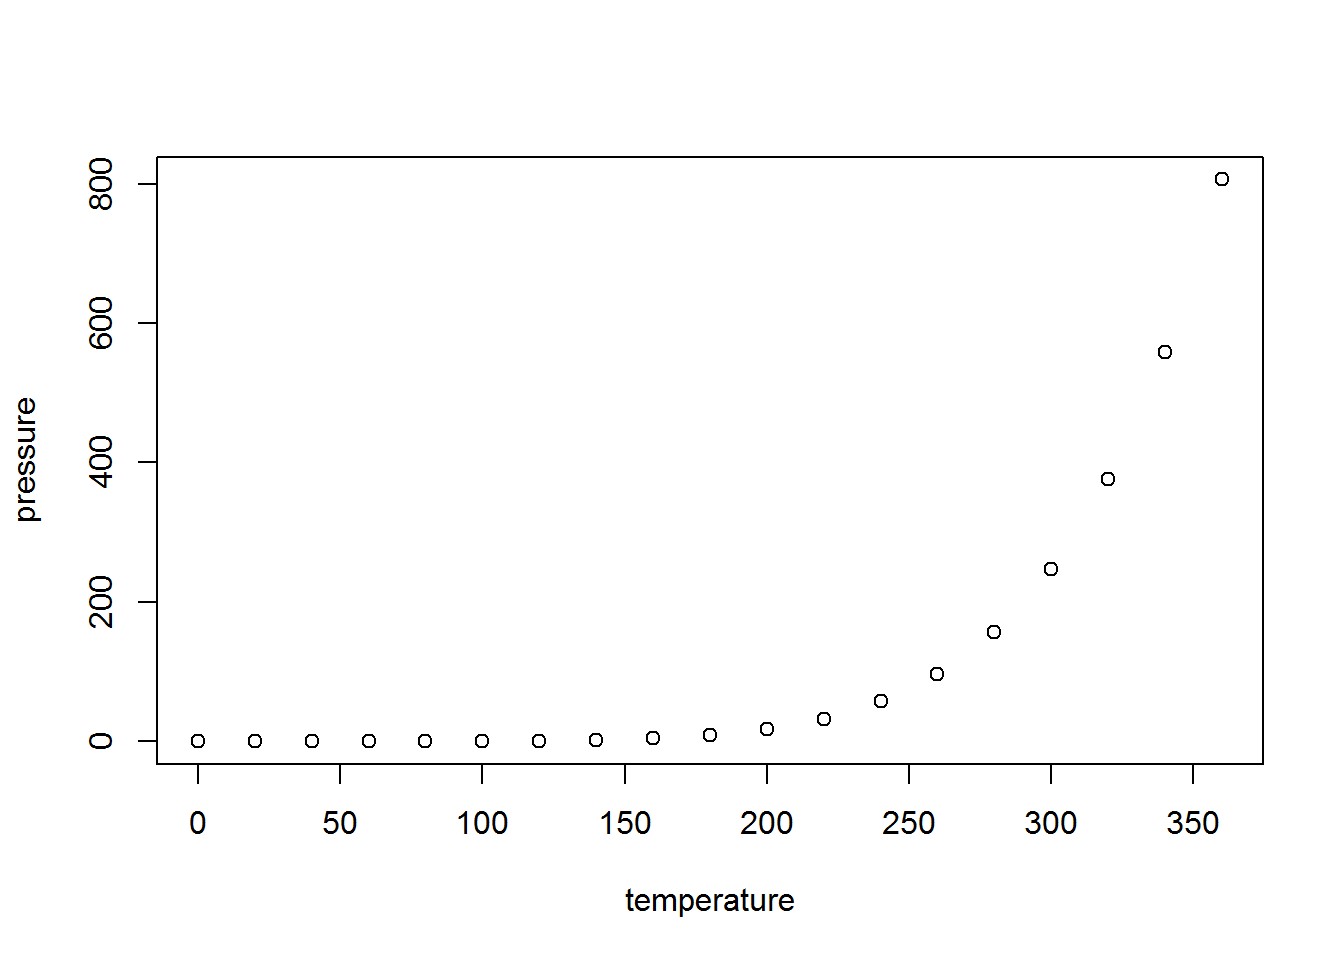
\includegraphics{1b-elastic-net-modelling_files/figure-latex/pressure-1.pdf}

\hypertarget{grid-search-results}{%
\subsection{Grid Search Results}\label{grid-search-results}}

\includegraphics{1b-elastic-net-modelling_files/figure-latex/unnamed-chunk-1-1.pdf}

\begin{Shaded}
\begin{Highlighting}[]
\KeywordTok{save.image}\NormalTok{(}\StringTok{"C:/Users/Peter/Desktop/ds_projects/betting_data_science/6 betting/1 model development/preliminary_data/1b elastic net modelling.RData"}\NormalTok{)}
\end{Highlighting}
\end{Shaded}

\end{document}
